\documentclass[a4paper,11pt]{article}
\usepackage[utf8]{inputenc}
\usepackage[usenames,dvipsnames]{color}
\usepackage{graphicx}
\usepackage[margin=1in]{geometry}
\usepackage[justification=centering,labelfont=bf]{caption}
\usepackage{listings}
\usepackage[hidelinks]{hyperref}
\usepackage{enumerate}

\makeatletter
\g@addto@macro\@floatboxreset\centering
\makeatother

\newcommand{\answerspace}{\vspace{0.5cm}}
\newcommand{\figurespace}{\vspace{0.6cm}}

\begin{document}
\begin{titlepage}
\begin{center}
\textsc{\Large Parallelism}
\\
\texttt{1202}
\\[1.5cm]
\rule{\linewidth}{0.5mm}
\\[0.4cm]
{\huge
\bfseries
Lab 1: Embracing parallelism with OpenMP: Mandelbrot set
\\[0.4cm]
}
\rule{\linewidth}{0.5mm}
\\[2.5cm]
\begin{minipage}{0.4\textwidth}
\begin{flushleft}
\large
Héctor Ramón Jiménez
\end{flushleft}
\end{minipage}
\begin{minipage}{0.4\textwidth}
\begin{flushright}
\large
Alvaro Espuña Buxo
\end{flushright}
\end{minipage}
\vfill
{\large
\today
}
\\
{\large
\texttt{Facultat d'Informàtica de Barcelona}
}
\end{center}
\end{titlepage}
\section{Reading activity}
In this first part of the report we first briefly describe the basic formulation for the \textbf{Mandelbrot set}
    (see \ref{mandelbrot:references}) and then its implementation in the sequential code available (\texttt{mandel-serial.c}).
\subsection{Description}
The \textbf{Mandelbrot set} is a particular set of points in the complex domain named after the mathematician
    \textbf{Benoit Mandelbrot}, who studied it and popularized it. The \textbf{Mandelbrot set}'s boundary is an easily
    recognizable two-dimensional fractal shape (see figure \ref{mandelbrot:boundary}).
\begin{figure}[h!]

\includegraphics[width=0.70\textwidth]{figures/mandelbrot_boundary.jpg}
\caption{The Mandelbrot set boundary}
\label{mandelbrot:boundary}
\end{figure}
\\
Mandelbrot set images are made by sampling complex numbers and determining for each whether the result
    \textbf{tends towards infinity} when a particular mathematical operation is \textbf{iterated} on it. The real
    and imaginary parts of each number are treated as image coordinates. The pixels are colored according to how rapidly
    the sequence diverges.
\\
More precisely, the \textbf{Mandelbrot set} is the set of values of $c$ in the complex plane for which the orbit of
    $0$ under iteration of the complex quadratic polynomial $z_{n+1} = z^2_n + c$ remains bounded.
\subsection{Algorithm}
The simplest algorithm for drawing a picture of the Mandelbrot set is the following. We \textbf{discretize} the
    complex space in a set of points and each point corresponds to a \textbf{pixel} in a two dimensional plot. To color
    any such pixel, let $c$ (represented by the complex variable $c$ at the \texttt{mandel-serial.c}
    code) be the midpoint of that pixel. Then we calculate $z_0$, $z_1$, ... (stored in the complex variable
    $z$) and beyond until \textbf{divergence} occurs or
    the \textbf{maximum number of iterations} is reached. We assume that divergence happens when the resulting complex
    $z_j$ is \textbf{not contained in the problem space}. More precisely, let the problem space be
    $\{ (r, i) \: | -\!N < r < N, \: -N < i < N \}$, then divergence occurs when:
\[
length(z_j) \geq N
\]
\\
The \textbf{intensity of the color} of the point $c$ is directly proportional to the \textbf{number of iterations performed}
    $k_c$ without divergence. Thus the points that belong to the \textbf{Mandelbrot set} are going to be the most intense ones
    (usually black color). That can be easily done calculating the \texttt{scale\_color} variable, which is the factor that needs
    to be applied to the \texttt{min\_color} for every performed iteration:
\[
\texttt{scale\_color}
=
\frac{\texttt{max\_color} - \texttt{min\_color}}{\texttt{maxiter} - 1}
\]
\[
\texttt{color}
=
(k_c - 1) \cdot \texttt{scale\_color} + \texttt{min\_color}
\]
\subsection{References}
\label{mandelbrot:references}
\begin{enumerate}
\item{Mandelbrot set - Wikipedia, the free encyclopedia. [Internet]. url:
    \url{http://en.wikipedia.org/wiki/Mandelbrot\_set} (visited on Apr 23, 2014).}
\end{enumerate}
\clearpage
\section{Task granularity analysis}
\begin{enumerate}
\setcounter{enumi}{0}
\item
\textbf{Which are the two most important common
    characteristics of the task graphs generated for the two task
    granularities (\emph{Row} and \emph{Point}) for
    \textbf{mandel-tareador}?  Include the task graphs that are
    generated in both cases for \texttt{-w 8}.}

\answerspace
The two most important characteristics we can see from both graphs are:
\begin{enumerate}[(1)]
  \item There are no data dependencies between tasks. They are fully parallelizable.
  \item There are tasks that take much more time (instructions) than
    others. Tasks are not homogeneus timewise.
\end{enumerate}

\begin{figure}[h!]
\includegraphics[width=0.7\textwidth, height=1.5cm]{figures/point_deps_mandel.pdf}
\caption{Task decomposition with \emph{Point} granularity.}
\label{figure:mandel-point}
\end{figure}

\begin{figure}[h!]
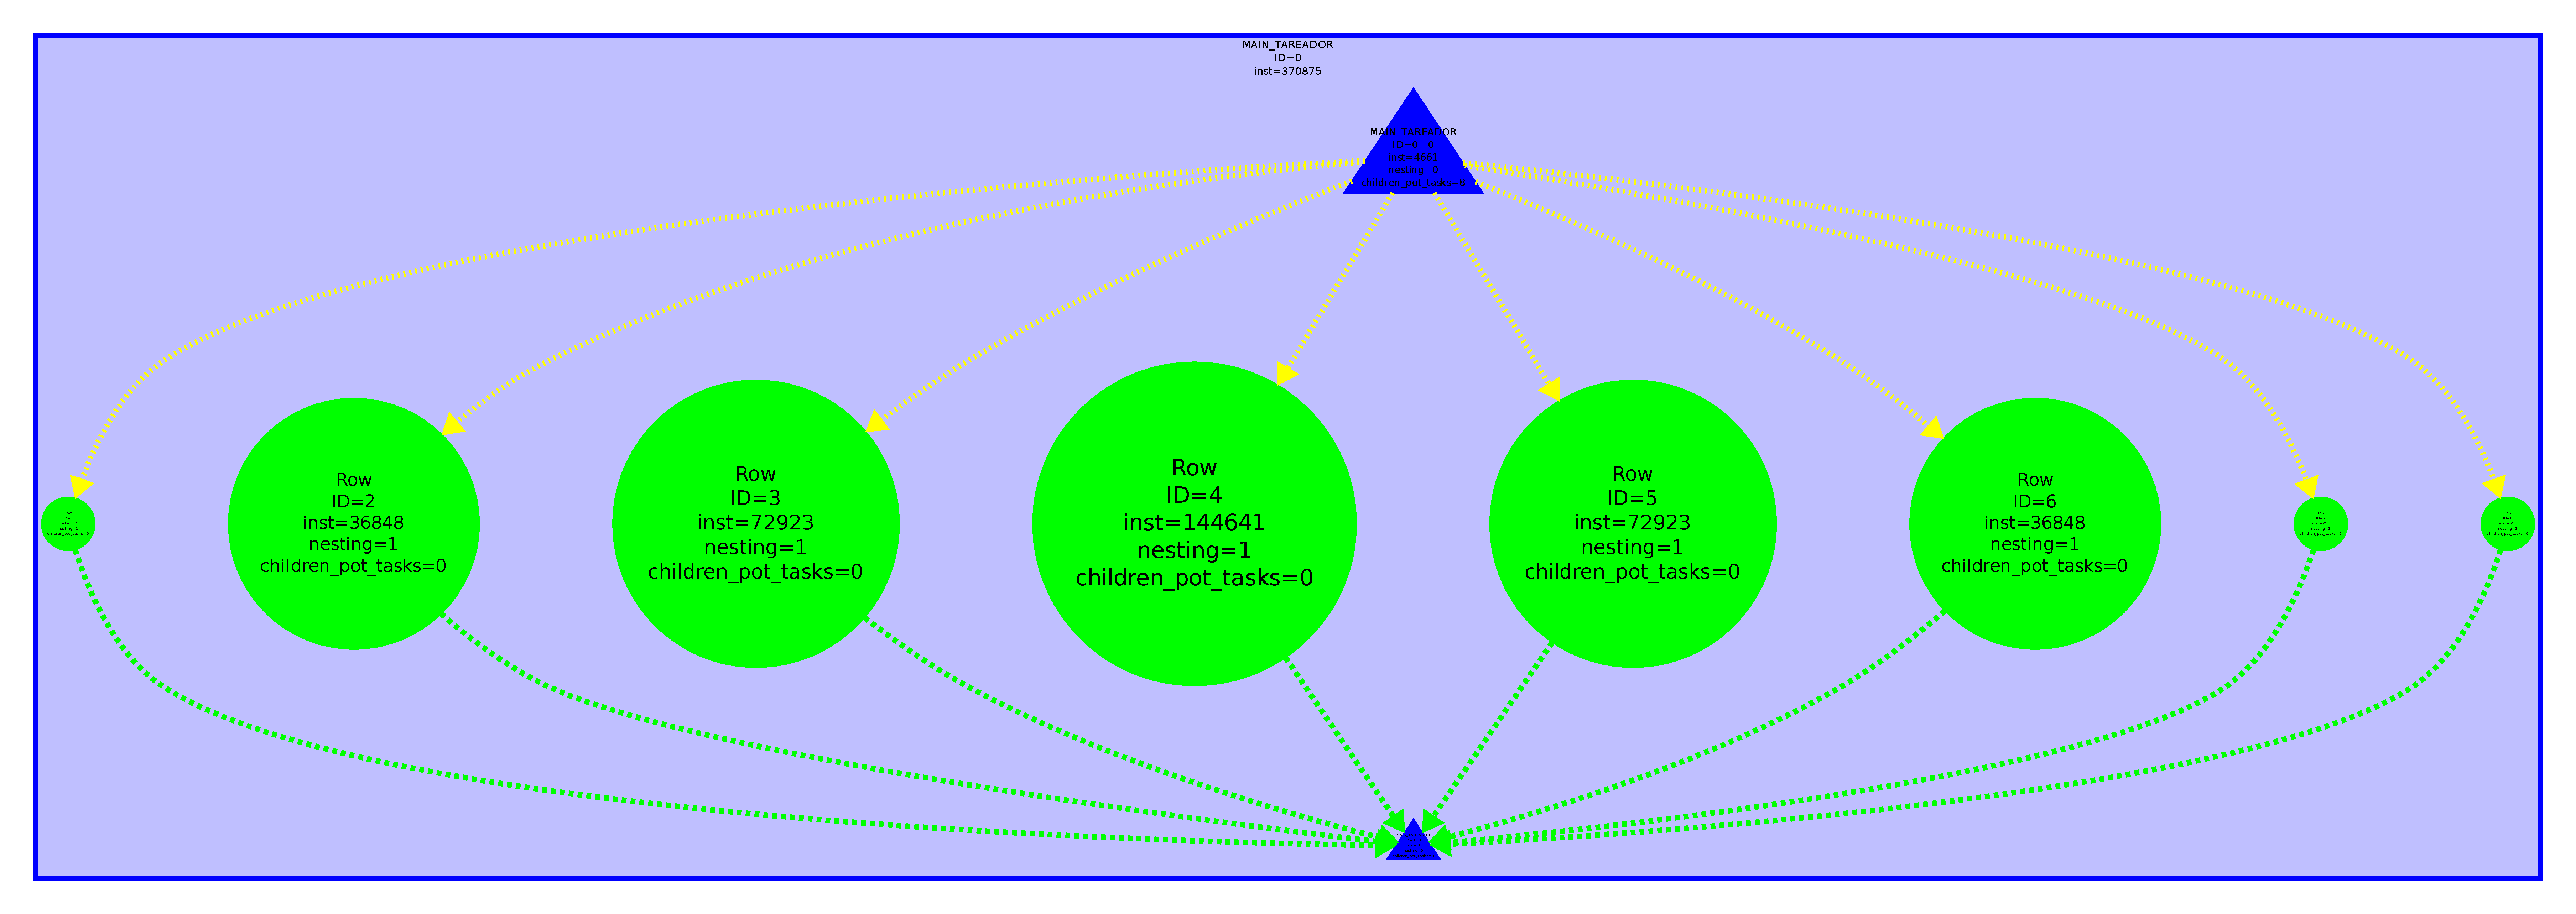
\includegraphics[width=0.7\textwidth]{figures/row_deps_mandel.pdf}
\caption{Task decomposition with \emph{Row} granularity.}
\label{figure:mandel-row}
\end{figure}

As we'll see later the different sizes of the tasks is very relevant in terms
of load balancing.

\newpage
\setcounter{enumi}{1}
\item
\textbf{Which section of the code is causing the serialization of
    all tasks in mandeld-tareador? Include the task graph generated for
    the graphical version of Point after isolating the section of the
    code}

The section that causes the serialization is the painting of the points. All threads
must wait after computing a point to paint it, since the display system doesn't allow
concurrent modifications of the window. The function \texttt{XDrawPoint} blocks
the execution, so tasks must be done serialized.

If we do \texttt{tareador\_disable\_object(display)} and
\texttt{tareador\_disable\_object(\&win)} we can parallelize it more:

\figurespace
\begin{figure}[h!]
\includegraphics[height=10cm]{figures/point_deps_mandeld.pdf}
\caption{mandeld after disabling the blocking objects.}
\label{figure:mandeld-point}
\end{figure}

In Figure \ref{figure:mandeld-point} we can see that it doesn't look
as parallel as \texttt{mandel}. It is more parallel than
\texttt{mandeld} without disabling nothing though. If we inspect data
dependencies in \emph{Tareador} we can see that there are still
dependencies, even when we disabled all the objects that present a
parallelism problem. The problem is in the function calls to the X
library. As we can not modify the library internals, we leave it this
way.

\newpage
\setcounter{enumi}{2}
\item
\textbf{Using the results obtained from the simulated parallel
    execution for mandel-tareador and for a size of -w 16, complete the
    following table with the execution time and speed-up (with respect to
    the execution with 1 processor) obtained for the non-graphical
    version, for both individual task granularities. Comment the results
    highlighting the reason for the poor scalability, if detected?}

\answerspace
  The results obtained of simulating the execution of
  \texttt{mandel-tareador} with \emph{Paraver} are:

  \figurespace
  \begin{center}
    \begin{tabular}{| c || c | c | c | c |}
      \hline
      & \multicolumn{2}{| c |}{\bf Row} & \multicolumn{2}{| c |}{\bf Point} \\
      \hline
      \textbf{Num. processors} & \textbf{Time (ms)} & \textbf{Speed-up} & \textbf{Time (ms)} & \textbf{Speed-up} \\
      \hline\hline
      \textbf{1} & 1080.584 & 1.000 & 1120.216 &  1.000 \\ \hline
      \textbf{2} &  554.698 & 1.948 &  563.475 &  1.988 \\ \hline
      \textbf{4} &  334.376 & 3.231 &  306.504 &  3.654 \\ \hline
      \textbf{8} &  330.156 & 3.272 &  163.536 &  6.849 \\ \hline
      \textbf{16} &  329.724 & 3.277 &   93.059 & 12.037 \\ \hline
    \end{tabular}
  \end{center}
  \figurespace
  We can see how \emph{Point} granularity seems to scale better than
  \emph{Row} granularity. At first, with two and four processors, we
  can see that both execution times are reduced and scale reasonably
  well, but as we add more processors, \emph{Row} stalls.

  The problem is that, with \emph{Row} granularity we have 16 tasks, and
  as we saw earlier, there are tasks that take a lot of time. We have a load balance
  problem, since some processor will have to execute the longest task while
  other processors are done and waiting. The longest row becomes the bottleneck,
  and adding more processors, won't produce speed-up.

  \figurespace
\begin{figure}[h!]
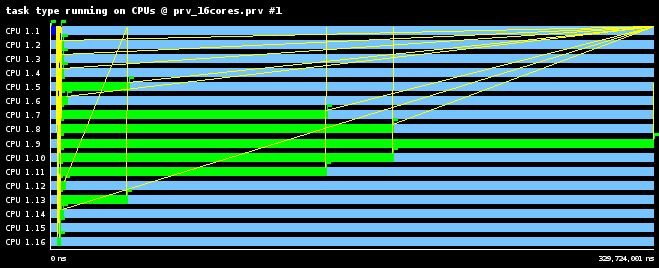
\includegraphics[width=0.7\textwidth]{figures/row_16_cores.png}
\caption{Row granularity: Most of the threads are in idle waiting for the longest task to finish.}
\label{figure:load-row}
\end{figure}
  \figurespace

  With \emph{Point} granularity, since we have 256 tasks ($16 \cdot 16$) while
  the longest points are being computed, the other processors can do other tasks,
  hence longest points are not the bottleneck now.

  \figurespace
\begin{figure}[h!]
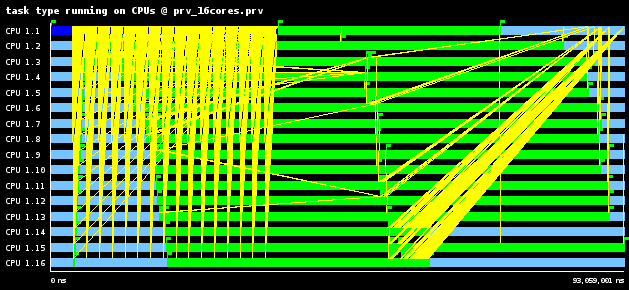
\includegraphics[width=0.7\textwidth]{figures/point_16_cores.png}
\caption{Point granularity: Since there are many more tasks than threads, the load can be distributed better.}
\label{figure:load-point}
\end{figure}
  \figurespace
  From this exercise we can conclude that when $n_{processors} <<
  n_{tasks}$ is more difficult to face load balance problems.

\end{enumerate}
\clearpage
\section{OpenMP execution analysis}
\begin{enumerate}
\setcounter{enumi}{3}
\item
\textbf{For each parallelization strategy of the non-graphical version, complete the following table with
    the execution time for different loop schedules and number of threads, reasoning about the results
    that are obtained.}

\answerspace
We did these exercise along with our colleagues of group 1201 (Lorenzo
Arribas and David Solà). They performed timing for the not \texttt{collapse}d version.
These are the results:

\begin{table}[h]
\begin{tabular}{| c || c | c | c | c |}
\hline
\textbf{Num. threads} & \textbf{static} & \textbf{static, 1} & \textbf{dynamic, 1} & \textbf{guided, 1}
\\
\hline
\hline
1 & 30.207 & 30.207 & 30.207 & 30.207
\\
\hline
2 & 15.223 & 15.233 & 15.206 & 15.224
\\
\hline
4 & 15.228 & 7.715 & 7.612 & 16.654
\\
\hline
6 & 14.716 & 5.391 & 5.334 & 11.438
\\
\hline
8 & 12.757 & 4.025 & 4.025 & 8.147
\\
\hline
10 & 10.924 & 3.364 & 3.376 & 7.127
\\
\hline
12 & 9.580 & 2.802 & 2.817 & 6.006
\\
\hline
\end{tabular}
\caption{Results for the uncollapsed version. Times are in seconds.}
\end{table}

\begin{itemize}
\item \texttt{static} gives the worst performance. This can be explained considering that
longest rows are contiguous, so a thread can have a chunk spanning multiple long
rows, increasing the length of the critical path.

\item \texttt{static,1} gives better results than \texttt{static} because rows are
  assigned one by one. This way, long rows end up being executed by different threads
  and can be more parallelized.

\item \texttt{dynamic,1} gives similar results as \texttt{static,1}. It's not important
  if threads are assigned dynamically or statically, since the bottleneck will be the same.
  The important thing is that chunks have size 1.

\item \texttt{guided,1} size of the chunks decreases as they are
  assigned to different threads. Because of this, we can see that with
  a low number of threads it behaves like \texttt{static} (since at
  the beginning chunks have size ${n_{tasks}}/{n_{threads}}$). At the
  end, though, as the chunk size decreases, it behaves better than
  \texttt{static}.

\end{itemize}

When using the \texttt{collapse} pragma we can only notice differences when the chunks
are big enough, otherwise they behave very similar to the uncollapsed version.
Having big chunks reduces the difference on the task sizes.

\newpage
\setcounter{enumi}{4}
\item
\textbf{For each parallelization strategy, complete the following table with the information extracted from
    the Extrae instrumented executions with 8 threads and analysis with Paraver, reasoning about the
    results that are obtained.}
\begin{center}
\begin{tabular}{| c || c | c | c | c |}
\hline
\textbf{} & \textbf{static} & \textbf{static, 1} & \textbf{dynamic, 1} & \textbf{guided, 1}
\\
\hline
\hline
Running avg. time per thread (s) & 3.800 & 3.986 & 3.984 & 3.872
\\
\hline
Execution balance & 0.298 & 0.986 & 0.998 & 0.459
\\
\hline
SchedForkJoin ($ms$) & 12667.786 & 70.510 & 0.504 & 7805.279
\\
\hline
\end{tabular}
\end{center}
[...]
\end{enumerate}
\end{document}
